%%
%% Copyright 2007, 2008, 2009 Elsevier Ltd
%%
%% This file is part of the 'Elsarticle Bundle'.
%% ---------------------------------------------

%% Please read the file, ``Addtional_AuthorInstruction_LaTeX.pdf'', for choosing the following options. 
%% Please choose only one of the two following options. Note that the option \final, which is also provided below, must not be submitted.
%\def\preprint{1}			% Use for submitted manuscript
\def\wordcount {1}		% Use for word count

%% The following option provides the final print version. This is only for personal use. Don't use this for submission.
%\def\final {1}			

%% Please do not modify the following nine lines
\ifdefined\preprint
  \documentclass[preprint,review,12pt]{elsarticle}
\fi
\ifdefined\wordcount
  \documentclass[final,3p,times,twocolumn]{elsarticle}
\fi
\ifdefined\final
  \documentclass[final,3p,times,twocolumn]{elsarticle}
\fi

%% Graphics packages for PostScript figures 
%% \usepackage{graphics}
\usepackage{graphicx,stfloats}
\usepackage{color}

\usepackage{blindtext}
\usepackage{latexsym,amsmath,amssymb}
\usepackage[T1]{fontenc}
\usepackage[utf8]{inputenc}
\usepackage[english]{babel}
\usepackage{csquotes}

\usepackage{algorithm2e}
\usepackage{scrextend}
\usepackage{mwe,tikz}
\usepackage[percent]{overpic}
%\pagestyle{empty}
\usepackage{color}
\usepackage[range-phrase={--},range-units=single]{siunitx}
\usepackage{graphicx}
\usepackage{tabularx}
\usepackage{subcaption}
\usepackage[export]{adjustbox}
\usepackage{wrapfig}
\usepackage{amsmath}
\graphicspath{{Figures/}}
\usepackage[version=4]{mhchem}
\usetikzlibrary{decorations.pathmorphing}
\tikzset{snake it/.style={decorate, decoration=snake}}

%% Other useful packages
\usepackage{booktabs,multirow,multicol}
% \usepackage{latexsym}
% \usepackage{subfigure}
% \usepackage{float}
% \usepackage{multirow}
% \usepackage{threeparttable}
%% The amssymb package provides various useful mathematical symbols
%\usepackage{amssymb}
%% The amsthm package provides extended theorem environments
%\usepackage{amsthm}

\usepackage{todonotes}

\biboptions{sort&compress}

\journal{Proceedings of the Combustion Institute}

\begin{document}

\begin{frontmatter}

\title{Assessing the importance of multicomponent transport properties using direct numerical simulations of premixed, high Karlovitz, turbulent flames}

\author[1]{Aaron J.~Fillo}

\author[2]{Jason Schlup}
\author[3]{Guillaume Blanquart}
\author[1]{Kyle E.~Niemeyer\corref{cor1}}
\ead{kyle.niemeyer@oregonstate.edu}

\address[1]{School of Mechanical, Industrial, and Manufacturing Engineering, Oregon State University, Corvallis, OR 97331, USA}
\address[2]{Graduate Aerospace Laboratories, California Institute of Technology, Pasadena, USA}
\address[3]{Mechanical Engineering, California Institute of Technology, Pasadena, USA}

\cortext[cor1]{Corresponding author:}

\begin{abstract}
Implementing multicomponent diffusion models in numerical combustion studies is computationally expensive due to the challenges involved in computing diffusion coefficients.
As a result, mixture-averaged diffusion treatments are used to avoid these costs.
However, to the authors' knowledge, the accuracy and appropriateness of the mixture-averaged diffusion models has not been verified for three-dimensional high Karlovitz turbulent premixed flames.
This study will evaluate the role of multicomponent mass diffusion in premixed, high Karlovitz hydrogen, n-heptane and toluene flames, neglecting secondary Soret and Dufour effects.
Direct numerical simulation (DNS) of these flames is performed by implementing the Stefan--Maxwell equations in NGA.
Premixed two-dimensional, unstable, and three-dimensional, turbulent hydrogen flames are simulated and compared with previous mixture-averaged DNS results.
Simulation conditions are carefully selected to match previously published results and ensure valid comparison.
A priori analysis shows similar relative angles and magnitudes between the species diffusion flux and species gradient vectors between mixture-averaged and multicomponent results.
Further, a posteriori analysis demonstrates negligible differences in conditional means of the fuel mass fraction and its diffusion source term against temperature for mixture-average and multicomponent transport, respectively, between the two cases.
\end{abstract}

\begin{keyword}
DNS \sep Turbulent Flame \sep Premixed \sep Diffusion \sep Multicomponent \sep Mixture Average
\end{keyword}

\end{frontmatter}


%% Please do not modify the following three lines
\ifdefined \wordcount
\clearpage
\fi

\section{Introduction}\label{Introduction}
% GB: Reacting flows have been performed with a wide range of diffusion models.  These include (in order of increasing complexity and accuracy): unity Lewis numbers, constant non-unity Lewis numbers, mixture average properties [REF], and ultimately multi-component [REF].
\textcolor{blue}{Leveraging simplified diffusion model formulations can be an effective way to reduce computational costs \cite{Xin:2015,Burali2016AssessmentFlows}.
Several diffusion models have been investigated in the past, including (in order of increasing accuracy and complexity) unity Lewis numbers, constant non-unity Lewis numbers, mixture-averaged properties \cite{Bird1960}, and multicomponent properties \cite{Hirschfelder1954}.
%Mixture-averaged diffusion models are commonly used to reduce the complexity of the governing system of equations by approximating the full multicomponent diffusion coefficient matrix as a diagonal matrix \cite{Bird1960}. 
%This approach reduces the the high computational expense associated with numerical combustion studies \cite{Burali2016AssessmentFlows}..
%Several approaches, such as those used by Warnatz \cite{Warnatz1978CalculationFlames} and Coltrin et al.~\cite{Coltrin1986ADeposition}, reduce the system's complexity even further by approximating multicomponent diffusion processes in terms of equivalent Fickian processes.  
%However, to the authors' knowledge, the accuracy and appropriateness of mixture-averaged approximations has not been evaluated for three-dimensional, moderate to high Karlovitz number (e.g. \numrange{140}{210}), turbulent flame simulations.
%GB: Lots of stuff on 1D and 2D flames...  This is marked as [2] in the pdf file.  I can talk about TD (i.e. Soret/Dufour) but only AFTER discussing some effects of MA vs MC.
%GB: For turbulent flames, the literature is spare
%%% 2
While data from three-dimensional reacting flow simulations with multicomponent transport are sparse, several studies have investigated the effects of multicomponent transport in simplified configurations.
These studies include one-dimensional \cite{Coffee:1981,Warnatz:1982, Ern:1999, Bongers:2003, Xin:2015} and two-dimensional flames \cite{Charentenay:2002}. 
These works include comparisons with various levels of diffusion and transport property modeling assumptions (from constant Lewis number to mixture-averaged properties).
In general, the result of these works indicate minor errors exist between multicomponent and mixture-averaged formulations, especially in simplified flame configurations, such as unstretched laminar flames.  
However, studies of three-dimensional turbulent flames frequently rely on simplified diffusion models and do not consider their accuracy to multicomponent diffusion.}

%Giovangigli \cite{Giovangigli2015MulticomponentFlames} demonstrated that multicomponent Soret effects significantly impact a wide range of laminar hydrogen/air flames.
%Specifically, they noted that multicomponent Soret effects influenced laminar flame speeds and extinction stretch rates for flat and strained premixed flames, respectively.

%Similarly, using a mechanistic approach, Yang et al.~\cite{Yang2010} observed that Soret diffusion of \ce{H} in premixed hydrogen flames actively modifies its concentration and distribution in the reaction zone.
%This effect was especially evident in symmetric, twin, counter-flow premixed hydrogen flames, where individual reaction rates could be increased in lean mixtures and decreased for rich mixtures coupled with Soret diffusion.
%Performing a similar mechanistic approach examining planar and stretched premixed \textit{n}-heptane and hydrogen flames, Xin et al.~\cite{Xin2012} demonstrated that these chemical kinetic effects were the result of dilution/enrichment of the reactant concentrations caused by Soret diffusion in the reaction front, and could have substantial impacts on the fuel burning rates especially in highly stretched flames.

%GB: Le=1 vs Le<>1.  This is the paragraph marked [4] in the pdf file.
\textcolor{blue}{Evaluations of diffusion models in three-dimensional simulations often involve comparisons between unity and constant, non-unity Lewis number approximations.
These studies are quite common, investigating a range of fuels, turbulence intensities, chemistry models, and flow configurations (e.g. \cite{Savard2015,Savard2015structure,Lapointe:2015,Burali2016AssessmentFlows}, among others).  
The results presented in these works indicate that, in many flame configurations with various fuel/air mixtures, differential diffusion effects can dramatically change the structure of the flame.}  %examining the normalized turbulent flame speeds, these difference were limited to differential diffusion.

%GB: Le <>1 vs MA.  This [5] in the pdf. 
\textcolor{blue}{Several studies have increased the complexity of diffusion models by exploring the differences between constant Lewis number and mixture-averaged transport processes \cite{Burali2016AssessmentFlows,Dinesh:2016,Aspden:2017}.
Among these works, Burali et al. \cite{Burali2016AssessmentFlows} demonstrated that the unity Lewis number assumption performed poorly relative to the constant, non-unity Lewis number and mixture-averaged diffusion models.}

% Thermal diffusion/Soret effects
\textcolor{red}{!!! Still don't like the location of this paragraph!!!}
\textcolor{blue}{One final example of the investigation of diffusion modeling is the impact of thermal diffusion.
Several studies have investigated the importance of including thermal diffusion in a wide range of flame configurations \cite{Coffee:1981,Ern:1998,Ern:1999,Bongers:2003,Yang2010,Xin2012,Dinesh:2016,Schlup2017}.
Contrary to the simplification from multicomponent to mixture-averaged mass diffusion found in simplified configurations, the neglect of thermal diffusion can have a significant impact on flame properties.  
While it is informative to acknowledge that thermal diffusion can be important in some fuel/air mixtures, its analysis is outside the scope of this work and is not considered further.}
% Conversely, Fillo et al.~\cite{Fillo2015,Fillo2017} experimentally observed significant differences between the normalized turbulent flame speeds of three jet fuel surrogates, with similar chemistry to the neat \textit{n}-heptane and isooctane flames studied by Lapointe and Blanquart \cite{Lapointe2016FuelFlames}.
% to better understand the mechanism responsible for these differences. 

% Several studies have investigated the impact of multicomponent transport for a wide range of simulations.
% For example, Dworkin et al.~\cite{Dworkin2009TheFlames} investigated the fidelity of the Fickian diffusion model for soot formation in ethylene/air flames.
% They showed that for low strain-rate flames, detailed multicomponent transport and thermal diffusion models reduce error in soot volume fractions in counter-flow diffusion flames.  

%GB: w/ vs w/o TD.  This is not here and could include Orszag (ask Jason) and Jason's CTM paper.
%\textcolor{red}{Further studies on the effects of thermal diffusion, implemented with mixture-averaged diffusion, have yielded similar results \cite{Grcar2009TheFlames,Schlup2017}.}

\textcolor{blue}{These results reinforce previous conclusions that differential diffusion effects can impact flame dynamics.
However, there has not been a detailed investigation of the accuracy and appropriateness of the mixture-averaged diffusion model relative to full multicomponent diffusion for turbulent reacting flows.
%GB: Then say that there is nothing about MA vs MC.  There is for non-reacting, that is [7], but not for reacting.  Make this clear.
For high-pressure systems, Borchesi et al.~\cite{Borghesi2015iAConditions} developed and analyzed a multi-species, turbulent mixing model for large eddy simulations of non-reacting flows.
They focused on turbulent crossflow mixing of a five-species combustion-relevant mixture which includes \textit{n}-heptane, \ce{O2}, \ce{CO2}, \ce{N2}, and \ce{H2O}.
This analysis showed that the multi-species transport model significantly improved the accuracy and fidelity of the solution throughout the mixing layer; however, as this study was restricted to non-reacting flows, it did not assess the impact of multicomponent transport on the stiff chemistry inherent in turbulent combustion. 
Thus, the observed discrepancies due to differential diffusion effects, and the lack of turbulent multicomponent reference data for reacting flows, warrant a detailed investigation of the fundamental transport phenomena involved.}

%These studies provide compelling evidence that multicomponent transport is important and can affect the accuracy of combustion models.
%However, these studies failed to assess the impact of multicomponent transport on three-dimensional systems with detailed chemistry.
%in regions of the mixing layer with strong gradients of density, temperature, and species mass fractions.
%%%%
% Add in discussion of scaling as motivation for simulation setup
%\begin{equation}
%    l_{D} = \frac{D_{i,j}}{(\nu\epsilon)^{1/4}},
%\end{equation}
%
%\begin{equation}
%    t_{D} = \frac{D_{i,j}}{(\nu\epsilon)^{1/2}},
%\end{equation}
%where,$l_{D}$ and $t_D$ are the diffusion time and length scales, $D_{i,j}$ is a representative diffusion coefficient, I propose the largest, $\nu$ is the viscosity, and $\epsilon$ is the turbulent dissipation rate.  Looking at the hydrogen case these values are comparable between Mixavg. and Multicomp. i.e. same order of magnitude.  I haven't done more on this yet but it's pretty straight forward.


%As noted previously, one- and two-dimensional simulations and non-reacting flows are often cited as a means of computational cost reduction.
% Motivated by the dearth of affordable three-dimensional multicomponent transport models, Ambikasaran and Narayanaswamy \cite{Ambikasaran2017AnVelocities} proposed an efficient algorithm to compute multicomponent diffusion velocities which scales as $\mathcal{O}(nSpecies)$.
% This offers a significant improvement over previous methods that directly invert the Stephan--Maxwell equations and scale as $\mathcal{O}(nSpecies^{3})$.

%\subsection{Objectives}
%GB: Then a real OBJECTIVE section (not an abstract)
\textcolor{blue}{The primary objective of this study is to evaluate the accuracy and appropriateness of the mixture-averaged diffusion assumption for use in direct numerical simulations (DNS) of premixed unsteady and turbulent flames.
This objective will be realized by a priori analyses of the diffusion fluxes given by the mixture-averaged and multicomponent formulations for a range of flame configurations.
%Freely propagating two-dimensional unsteady hydrogen/air flames, and three-dimensional, turbulent, premixed \textit{n}-heptane, toluene, and hydrogen/air flames are simulated.
%An a priori analysis of the magnitude and direction of species flux vectors is performed to assess the relative differences between mixture-averaged and multicomponent species diffusion transport.
Additionally, a posteriori results will help analyze the effects of diffusion modeling assumptions on species transport and chemical source terms in turbulent flames.
%An a posteriori analysis of the mean fuel mass fractions and source terms are performed to determine the relative impact of differential diffusion effects on the turbulent characteristics of these flames.
% \textcolor{red}{assessment of the impact of mixture-averaged and multicomponent mass diffusion transport on the turbulent statistics of the three-dimensional simulations is presented.}
% \textcolor{red}{an a priori and a posteriori assessment of the importance of multicomponent transport using DNS of turbulent, premixed, high Karlovitz flames within the flamelet regime.
% Freely propagating two-dimensional unsteady, and three-dimensional, turbulent, premixed flames are simulated.}
%\subsection{Outline}
%GB: Finally, an outline...
The paper is organized as follows: the governing equations, diffusion models, and flow configurations for the simulations are described in Section \ref{sec:numericalapproach}.
Then, the results from a priori and a posteriori analyses are presented in Section \ref{sec:results}.
Finally, Section \ref{sec:conclusions} draws conclusions from the comparisons of the diffusion models.}

\section{Numerical approach}\label{sec:numericalapproach}
In this section, a description of the reacting flow equations is given, including brief discussions of the diffusion models to be studied. The two- and three-dimensional flow configurations used are presented.

\subsection{Governing equations}
The variable-density, low Mach number, reacting flow equations are solved using
the finite-difference code NGA \cite{Desjardins2008,Savard2015AChemistry}.
The conservation equations are
%
\begin{equation} \label{1}
\frac{\partial\rho}{\partial t}+\nabla\cdotp(\rho\textbf{u})= 0 \;,
\end{equation}
%
\begin{equation} \label{2}
\frac{\partial\rho \textbf{u}}{\partial t}+\nabla\cdotp(\rho\textbf{ u}\otimes\textbf{u})=-\nabla p+\nabla\cdotp\boldsymbol{\tau}+\textbf{f} \;,
\end{equation}
%
\begin{equation} \label{3}
\begin{split}
\frac{\partial\rho T}{\partial t}+\nabla\cdotp(\rho \textbf{u}T)=\nabla\cdotp(\rho\alpha\nabla T)+\rho\dot{\omega}_{T}\\
-\frac{1}{c_{p}}\sum_{i} c_{p,i}\textbf{j}_{i} \cdotp \nabla T+\frac{\rho\alpha}{c_{p}}\nabla{c_{p}}\cdotp\nabla T \;,
\end{split}
\end{equation}
%
\begin{equation} \label{4} 
\frac{\partial\rho Y_{i}}{\partial t}+\nabla\cdotp(\rho \textbf{u} Y_{i})=-\nabla\cdotp \textbf{j}_{i}+\rho\dot{\omega_{i}} \;,
\end{equation}
where $\rho$ is the mixture density, $\textbf{u}$ is the velocity, $p$ is the hydrodynamic pressure, $\boldsymbol{\tau}$ is the viscous stress tensor, $\textbf{f}$ represents volumetric forces, $T$ is the temperature, $\alpha$ is the mixture thermal diffusivity, $c_{p,i}$ is the constant-pressure specific heat of species $i$, $c_{p}$ constant-pressure specific heat of the mixture, $\textbf{j}_{i}$ is the diffusion flux of species $i$, $Y_{i}$ is the mass fraction of species $i$, and $\dot{\omega_{i}}$ is the production rate of species $i$.
In Eq. \eqref{3}, the temperature source term is given by
\begin{equation} \label{5}
\dot{\omega}_{T}=-c_{p}^{-1}\sum_{i} h_{i}(T)\dot{\omega_{i}} \;,
\end{equation}
where $h_{i}(T)$ is the specific enthalpy of species $i$ as a function of temperature.
The density is determined from the ideal gas equation of state.

\subsection{Overview of diffusion models}
The diffusion fluxes are calculated with both the mixture-averaged \cite{Bird1960} and multicomponent \cite{Hirschfelder1954} models, which are both based on Boltzmann's equation for the kinetic theory of gases \cite{Curtiss1949TransportMixtures, Hirschfelder1954, Chapman1970, Ferziger1972, Lam2006MulticomponentRevisited}.
\textcolor{blue}{For this study, both baro-diffusion and thermal diffusion (Soret and Dufour effects) are neglected.
The baro-diffusion term is commonly neglected in reacting flow simulations under the low Mach number approximation \textcolor{red}{\cite{Grcar2009TheFlames}}.
Thermal diffusion has also been neglected as the objective of this work is to investigate the impact of only mass diffusion models; the effects of thermal diffusion model assumptions have been explored in ~\cite{Schlup2017}.}

The species diffusion flux for the mixture-averaged diffusion model is related to the species gradients by a Fickian formulation and is expressed as
\begin{equation}\label{6}
\textbf{j}_{i}^{MA}=-\rho D_{im}\frac{Y_i}{X_{i}}\nabla X_{i}+\rho Y_{i}\textbf{u}_{c}' \;,
\end{equation}
where $X_i$ is the $i$th species mole fraction, $D_{i,m}$ is the $i$th species mixture-averaged diffusion coefficient as expressed by Bird et al.~\cite{Bird1960},
\begin{equation}\label{7}
D_{im}=\frac{1-Y_{i}}{\sum_{i\neq j}^{N} X_{j}/\mathcal{D}_{ji}} \;,
\end{equation}
where $\mathcal{D}_{ji}$ is the binary diffusion coefficient of species $i$ and $j$, and $\textbf{u}_{c}$ is the correction velocity used to ensure mass continuity:
\begin{equation} \label{8}
\textbf{u}_{c}=\sum_{i}\rho D_{im}\frac{Y_{i}}{X_{i}}\nabla X_{i} \;.
\end{equation}

Alternatively, the multicomponent diffusion model for the species diffusion flux as presented by Bird et al.~\cite{Bird1960} and implimented in CHEMKIN II \cite{Kee1989Chemkin-II:Kinetics} is
\begin{equation} \label{9}
\textbf{j}_{i}^{MC}=\frac{\rho Y_{i}}{X_{i}W}\sum_{i\neq j}^{N}W_{j}D_{i,j}\nabla{X_{j}} \;,
\end{equation}
where $W$ is the mixture molecular weight, $W_{j}$ is the molar mass of the $j$th species, and $D_{i,j}$ is the ordinary multicomponent diffusion coefficient computed using the \texttt{MCMDIF} subroutine of CHEMKIN II~\cite{Kee1989Chemkin-II:Kinetics} with the method outlined by Dixon-Lewis~\cite{Dixon-Lewis1968FlameSystems}.

\begin{table*}[htb]
    \caption{Parameters of the simulations.  $L$ is the domain size in the spanwise direction, $\Delta x$ is the grid spacing, $\eta_{u}$ is Kolmogorov length scale in the unburnt gas, $\Delta t$ is the simulation time step, $\phi$ is the equivalence ratio, $T_{peak}$ is the temperature of peak fuel consumption rate in the one-dimensional laminar flame, $S_L$ is the laminar flame speed, $l_F = \left(T_b - T_u\right)/\left|\nabla T\right|_{max}$ is the laminar flame thickness, $l = u'^3/\epsilon$ is the integral length scale, $u'$ is the turbulence fluctuations, $\epsilon$ is the turbulent energy dissipation rate, $Ka_u$ is the Karlovitz number in the unburnt mixture, $Re_t$ is the turbulent Reynolds number in the unburnt mixture, and $\nu_u$ is the unburnt kinematic viscosity.}
    \centering
    \begin{tabularx}{\textwidth}{@{\extracolsep{\fill}}l c c c c c c c c@{}}
         \toprule
         & \multicolumn{2}{c}{\ce{H2} (2D)} & \multicolumn{2}{c}{\ce{H2}} & \multicolumn{2}{c}{\textit{n}-\ce{C7H16}} & \multicolumn{2}{c}{\ce{A1CH3}} \\
         \midrule
         & MA & MC & MA & MC & MA & MC & MA & MC \\
         \midrule
         Domain & \multicolumn{2}{c}{$4L \times L$}  & \multicolumn{2}{c}{$8L \times L \times L$} & \multicolumn{2}{c}{$11L \times L \times L$} & \multicolumn{2}{c}{$11L \times L \times L$} \\
         L & \multicolumn{2}{c}{$472\Delta{x}$} & \multicolumn{2}{c}{$190\Delta{x}$} & \multicolumn{2}{c}{$128\Delta{x}$} & \multicolumn{2}{c}{$128\Delta{x}$} \\
         Grid & \multicolumn{2}{c}{$1888\times472\times1$}  & \multicolumn{2}{c}{$1520\times190\times190$} & \multicolumn{2}{c}{$1408\times128\times128$} & \multicolumn{2}{c}{$1408\times128\times128$} \\
         $\Delta{x}$ [\si{\mm}] & \multicolumn{2}{c}{$0.0424$} & \multicolumn{2}{c}{$0.0424$} & \multicolumn{2}{c}{$1.8\times10^{-5}$} & \multicolumn{2}{c}{$1.8\times10^{-5}$} \\
         $\eta_{u}$ [\si{\m}] & \multicolumn{2}{c}{---} & \multicolumn{2}{c}{$2.1\times10^{-5}$} & \multicolumn{2}{c}{$9.0\times10^{-6}$} & \multicolumn{2}{c}{$9.1\times10^{-6}$} \\
         $\Delta{t}$ [\si{\s}] & \multicolumn{2}{c}{$5\times10^{-6}$} & \multicolumn{2}{c}{$6\times10^{-7}$} & \multicolumn{2}{c}{$6\times10^{-7}$} & \multicolumn{2}{c}{$6\times10^{-7}$} \\
         $\phi$ & \multicolumn{2}{c}{$0.4$} & \multicolumn{2}{c}{$0.4$} & \multicolumn{2}{c}{$0.9$} & \multicolumn{2}{c}{$0.9$} \\
         $T_{peak}$ [\si{\K}] & $1190$ & $1180$ & $1190$ & $1180$ & $1270$ & $1230$ & $1490$ & $1490$ \\
         $S_{L}$ [\si{\m\per\s}] & $0.230$ & $0.223$ & $0.230$ & $0.223$ & $0.351$ & $0.373$ & $0.343$ & $0.344$ \\
         $l_{F}$ [\si{\mm}] & $0.643$ & $0.651$ & $0.643$ & $0.631$ & $0.39$ & $0.385$ & $0.41$ & $0.42$ \\
         $l/l_{F}$ & \multicolumn{2}{c}{---} & $2$ & $2.04$ & $1.1$ & $1.1$ & $1.1$ & $1.1$ \\
         $u'/S_{L}$ & \multicolumn{2}{c}{---} & $18$ & $18.6$ & $18$ & $16.9$ & $17$ & $16.9$ \\
         $Ka_{u} = \tau_{F}/\tau_{\eta}$ & \multicolumn{2}{c}{---} & $149$ & $151$ & $220$ & $207$ & $200$ & $204$ \\
         $Re_t = (u'l)/\nu_{u}$ & \multicolumn{2}{c}{---} & \multicolumn{2}{c}{$289$} & \multicolumn{2}{c}{$190$} & \multicolumn{2}{c}{$175$}  \\
         \bottomrule
    \end{tabularx}
    \label{tab:3D_flow_config}
\end{table*}

\subsection{Flow configuration}
\textcolor{red}{!!! Why do we have 2D and 3D flames under high Ka? !!!}
Two flow configurations are used in this work.  The first is a two-dimensional domain used to study unsteady, freely propagating lean hydrogen/air flames \cite{Burali2016AssessmentFlows,Schlup2017}.  The second configuration is a doubly-periodic domain used to study three-dimensional statistically stationary flames \cite{Burali2016AssessmentFlows,Lapointe2016FuelFlames,Schlup2017}.
\textcolor{blue}{Both configurations have been used in previous studies; only a brief overview is provided here.}
\subsubsection{Two-dimensional flow configuration}\label{sec:twoDconfig}
% A similar configuration has been used to investigate two-dimensional freely-propagating flames~\cite{Grcar2009TheFlamesb,Bastiaans2012NumericalCombustion,Regele2013AFlames}, while this exact configuration was used in~\cite{Burali2016AssessmentFlows,Schlup2017}.  
% Only a brief discussion is given here.
%The flame is initialized with an array of solutions corresponding to the one-dimensional flat flame simulations run previously, with an equivalence ratio of $\phi=0.4$ and an inlet temperature and pressure of \SI{298}{\kelvin} and \SI{1}{atm}, respectively.
% The flame profile is initially perturbed in the span-wise direction by two sinusoidal modes.
\textcolor{blue}{The two-dimensional analysis is performed using only the hydrogen/air mixture, with nine species, 54 reaction chemistry model of Hong et al.~\cite{Hong2011AnMeasurements,Lam2013AAbsorption,Hong2013OnAbsorption} (forward and backward reactions counted separately).  The domain has inlet and convective outlet boundaries in the streamwise directions and periodic boundaries in the spanwise direction.
The inlet velocity boundary condition is fixed at the mean effective burning velocity, such that the unstable flame remains statistically stationary in the domain.}  The mean effective burning velocity $S_{\text{eff}}^{2D}$, defined as:
\begin{equation}
S_{\text{eff}}^{2D}=-\frac{\int_{A} \rho \dot{\omega}_{\ce{H2}} dA}{\rho_{u} Y_{\ce{H2},u} L} \;,
\end{equation}
where $L$ is the spanwise dimension of the computational domain.
This velocity boundary condition allows the simulation to run for an arbitrary time, while keeping the unstable flame within the domain.
\begin{figure}[!tb]
\centering
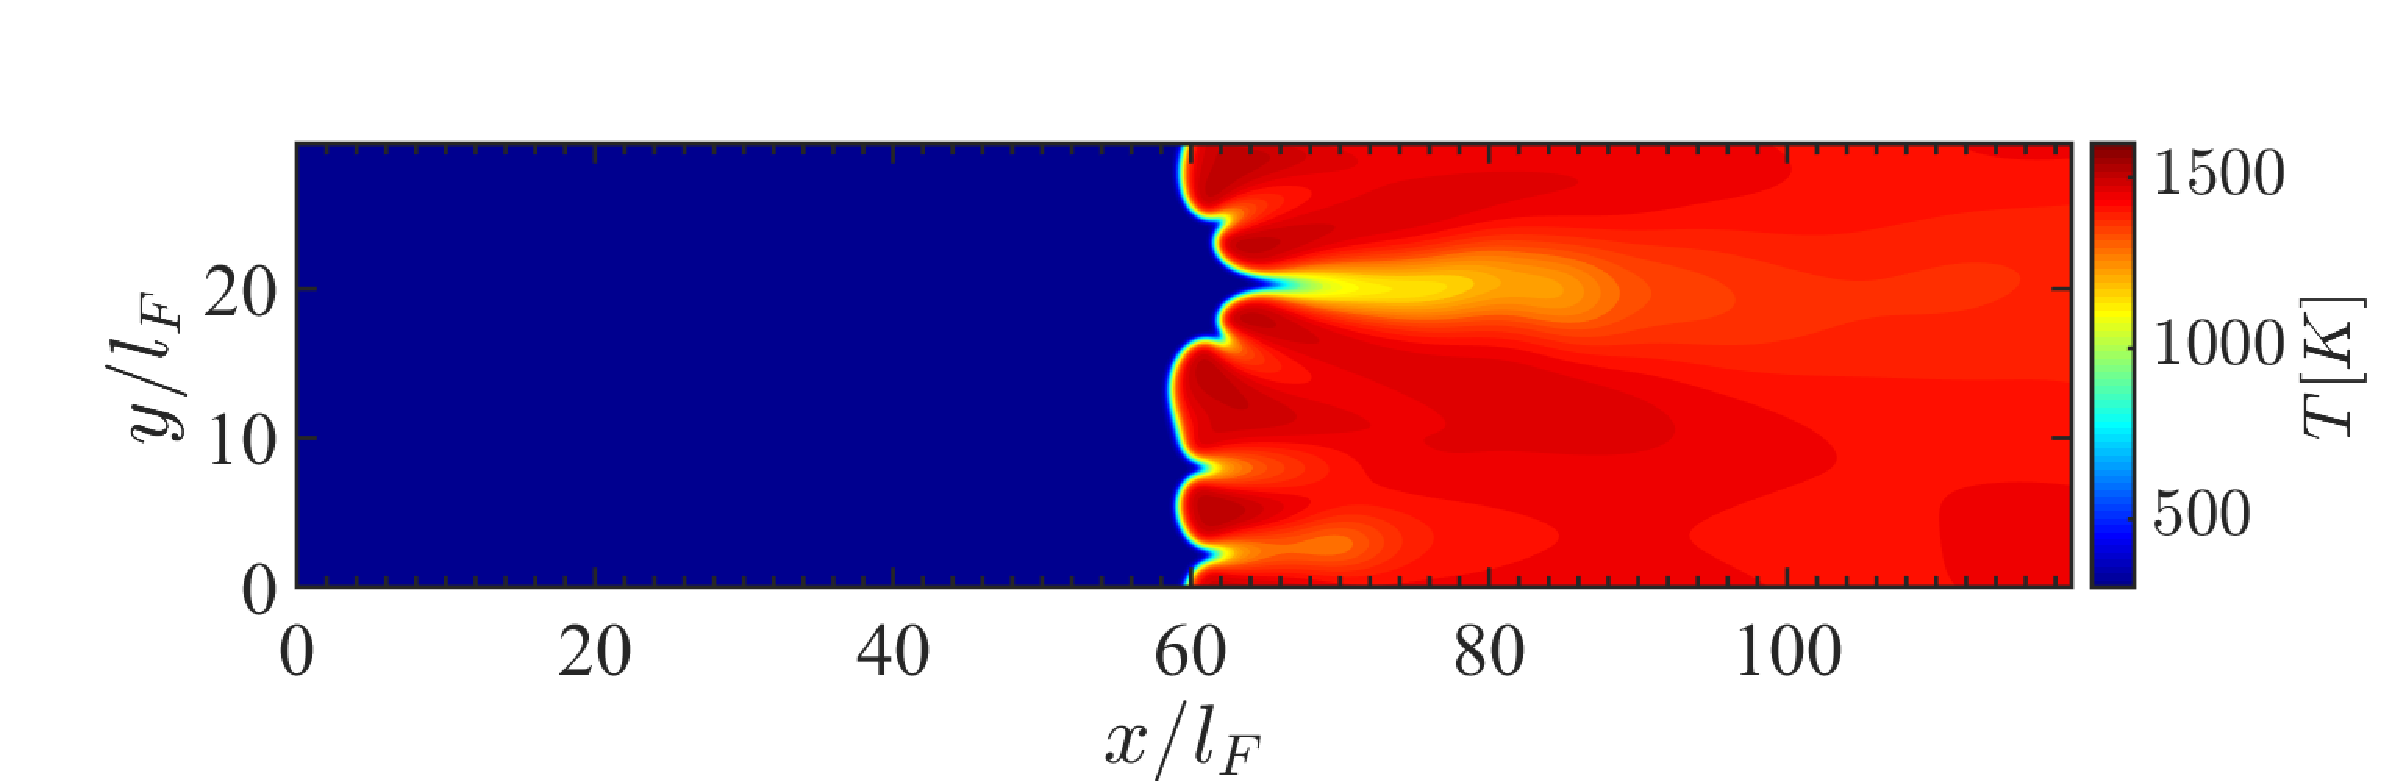
\includegraphics[trim={1.75cm 0 0 2cm},clip,width=\columnwidth]{2D_flame_temp.pdf}
\caption{Temperature contour for the two-dimensional freely propagating unsteady hydrogen/air flame obtained with the multicomponent diffusion model.} \label{2D_temp}
\end{figure}
The physical size of the domain is approximately \SI{120}{\textit{l}_{\textit{F}}} in the stream-wise direction by \SI{30}{\textit{l}_{\textit{F}}} in the spanwise direction.
The grid is a structured, uniform mesh with $1888 \times 472$ cells, with a cell size corresponding to $\Delta x = \Delta y = l_{F}/16$.
The unburnt mixture has an equivalence ratio of $\phi = 0.4$, unburnt temperature of $T_u = 298\,\rm K$, and unburnt pressure of $p_o = 1\,\rm atm$.
Details of the unstable flame initialization are given in Burali et al. \cite{Burali2016AssessmentFlows}.
Figure~\ref{2D_temp} shows an example temperature contour with a representative usnteady flame clearly visible.

\subsubsection{Three-dimensional flow configuration}\label{sec:threeDconfig}
% The three-dimensional turbulent flames are simulated using an identical flow configuration as previous works \cite{Savard2015,Burali2016AssessmentFlows,Schlup2017}, thus only a brief description is provided.
\textcolor{blue}{Three fuel/air mixtures are simulated in the three-dimensional cases.  The hydrogen/air mixture uses the chemical model described in Section \ref{sec:twoDconfig}.  
The heptane/air mixture uses the 35 species, 217 reaction reduced chemical model of Bisetti et al. \cite{mech35} (aromatic species have been removed).
Finally, the toluene/air mixture uses the 47 species \textcolor{red}{!!! Describe RedMech 47 with [REF]!!!}}

The computational domain consists of inflow and convective outflow boundary conditions in the streamwise direction.  
In the two spanwise directions, periodic boundaries are implemented. 
The inflow velocity is set as the mean turbulent flame speed to keep the flame statistically-stationary such that turbulent statistics can be collected over an arbitrarily long run time.
In the absence of mean shear, a linear turbulence forcing method \cite{Rosales2005,Carroll2013} is implemented in order to maintain the production of turbulent kinetic energy through the flame.
The unburnt temperatures and pressures for each case are $298\,\rm K$ and $1\,\rm atm$, respectively.
Further details of the computational domain, unburnt mixture, corresponding one-dimensional flames, and inlet turbulence are defined in Table \ref{tab:3D_flow_config}.
\textcolor{blue}{Note that definitions of the Karlovitz number, $Ka_u$, and turbulent Reynolds number, $Re_t$, are also given in Table \ref{tab:3D_flow_config}, where $\tau_F = l_F/S_L$ is the flame time scale and $\tau_{\eta}=\left(\nu_u/\epsilon\right)^{1/2}$ is the Kolmogorov time scale of the incoming turbulence.}

\section{Results and discussion}\label{sec:results}
% Update stub header
This section presents a priori results for the two-dimensional, unsteady, premixed hydrogen/air flame, as well as a priori and a posteriori results for the three-dimensional, turbulent, premixed hydrogen, \textit{n}-heptane, and toluene flames.

\subsection{A priori diffusion flux comparison}\label{sec:aprioriresults}

\textcolor{blue}{The a priori analysis is performed using data files obtained from the multicomponent simulations and used to evaluate the mass fluxes corresponding to each model;} this was done to isolate the effects of the diffusion model from any time evolution of the reacting flow field.
The a priori assessment of the agreement between mixture-averaged and multicomponent diffusion fluxes is presented in two parts.
The relative angles of the flux vectors are investigated due to the the mathematical definitions of the two diffusion models. 
As demonstrated in Eq.~\eqref{6}, the mixture-averaged flux vector for species $i$ is based on the gradient of that species and, as a result, must be anti-parallel to the species gradient vector.
Alternatively, in Eq.~\eqref{9}, the multicomponent flux of species $i$ is based on the net influence of the other $n-1$ species (but not itself) and thus may not necessarily align with its own species gradient vector.

Figure~\ref{A priori (a)} presents the probability density function (PDF) of the angle between the species diffusion flux vector and species gradient vector for the mixture-averaged and multicomponent models \textcolor{red}{in the two-dimesional configuration}.
\textcolor{red}{Only points for which the species diffusion flux magnitude is 0.1\% of the peak species diffusion flux magnitude in the domain are considered, to emphasize the region where diffusion is important}.
Note that only results for \ce{H2} are given in Fig.\ref{A priori (a)}, while compiled results for various major, radical, and product species are presented in Table \ref{tab:L2_norms}.
%To ensure a one-to-one comparison, the a priori analysis was run with identical data files for both the mixture-averaged and multicomponent models; 


\begin{figure*}[htb]
    \begin{subfigure}{0.33\textwidth}
        \centering
            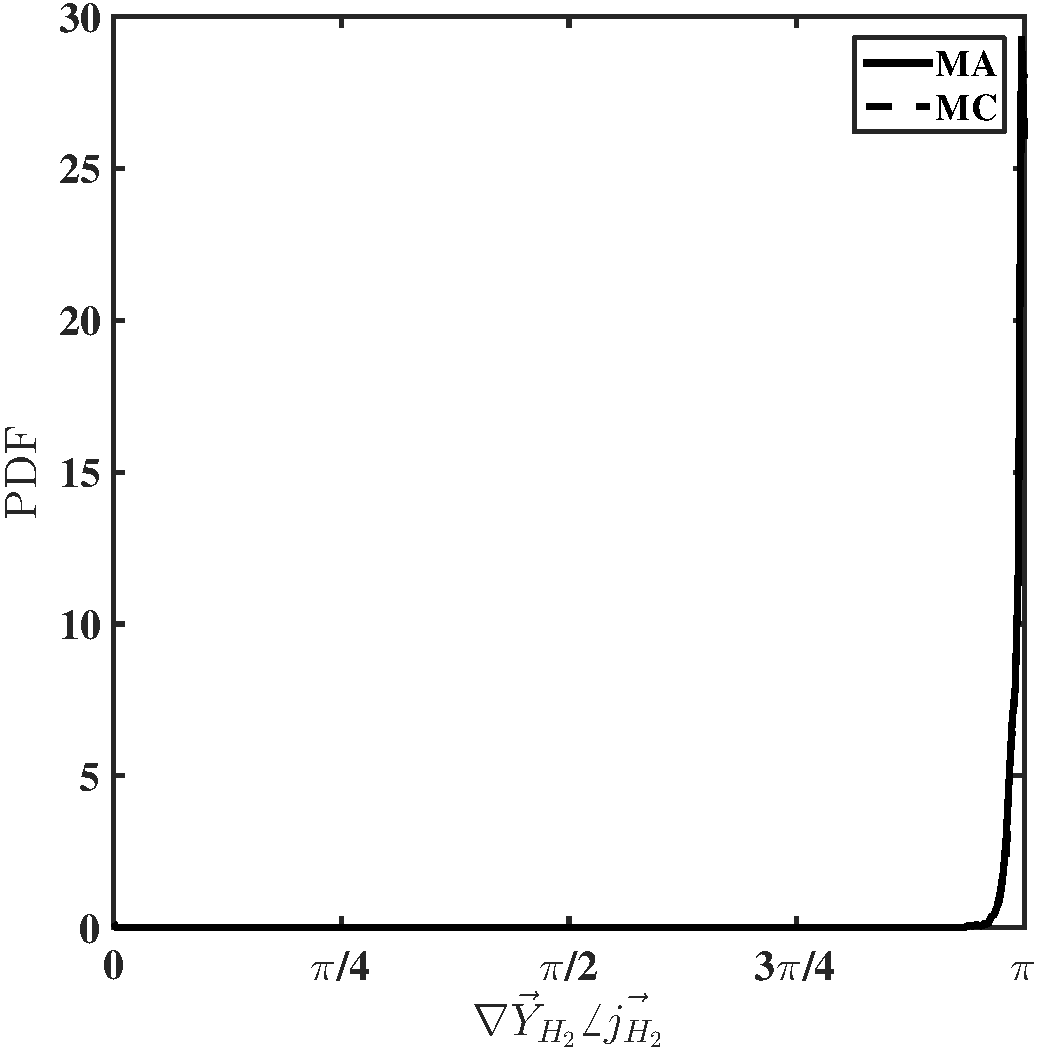
\includegraphics[width=\textwidth]{Angle_PDF.pdf}
        \caption{}\label{A priori (a)}
    \end{subfigure}
    \begin{subfigure}{0.33\textwidth}
        \centering
            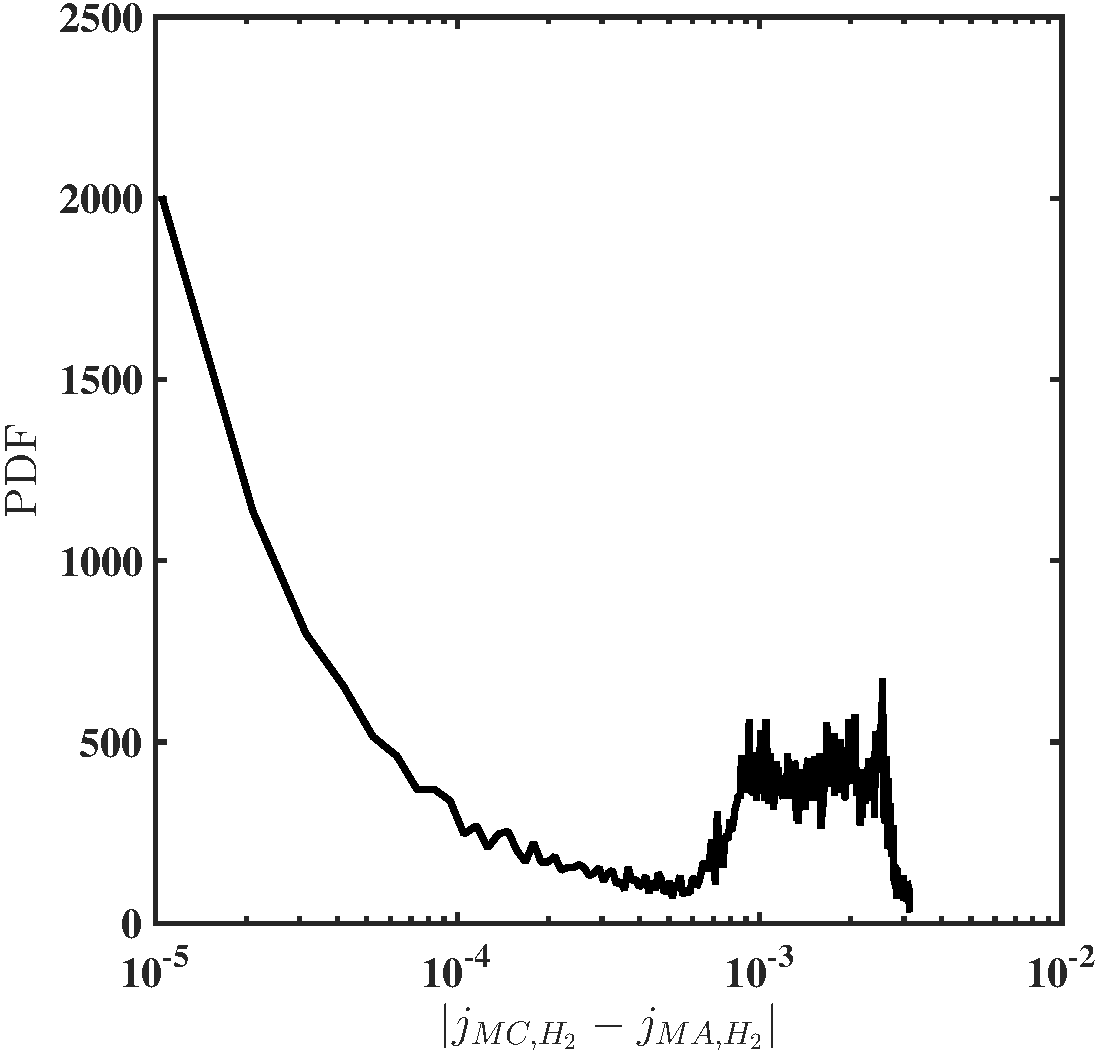
\includegraphics[width=\textwidth]{Flux_diff_PDF.pdf}
        \caption{}\label{A priori (b)}
    \end{subfigure}
    \begin{subfigure}{0.33\textwidth}
        \centering
        \begin{tikzpicture}[overlay]
            \node at (0,0.2) {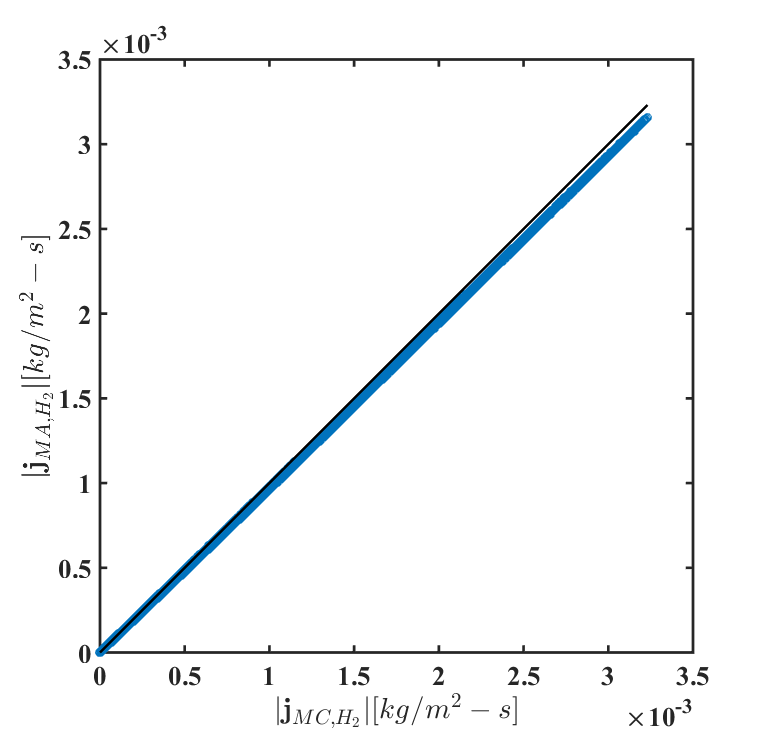
\includegraphics[width=1.075\textwidth]{H2_flux_scatter_linear.png}};
            \node at (0.8,0.0) {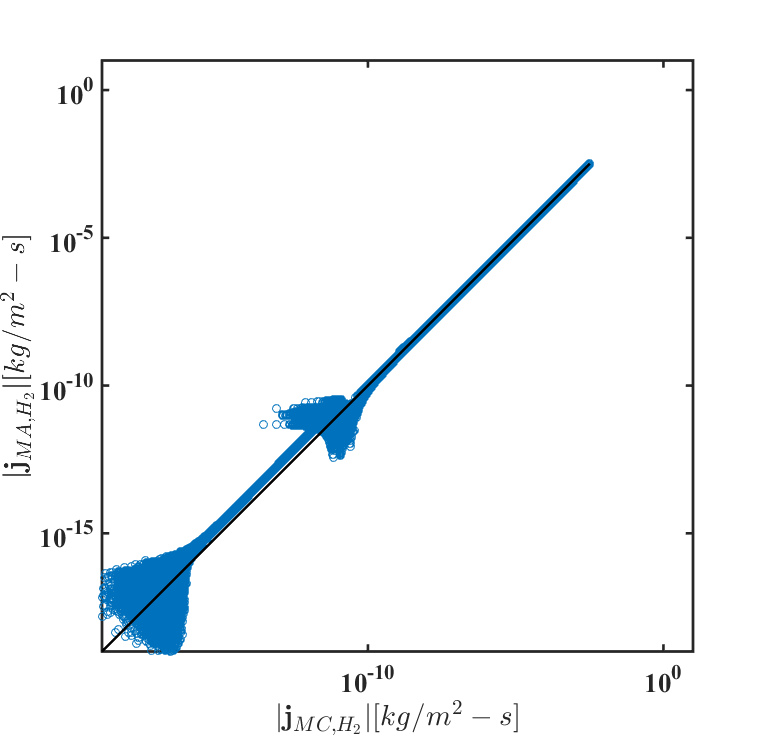
\includegraphics[width=0.5\textwidth]{H2_flux_scatter.png}};
        \end{tikzpicture}
        \caption{}\label{A priori (c)}
    \end{subfigure}
  \caption{A priori assessment of the mixture-averaged and multicomponent models comparing: (a) the PDFs of the angle between species flux vectors and species gradient vectors, (b) the PDF of the difference between magnitudes of the fluxes, and (c) a scatter plot of the multicomponent vs mixture-averaged fluxes for \ce{H2} (black line is unity case, i.e. $y=x$). Inset plots are log-log scale. \textcolor{red}{FIX PLOT Resolution}}\label{A priori}
\end{figure*}

\textcolor{red}{!!! Redo with new angle analysis!!!}  Both mixture-averaged and multicomponent diffusion models have maximum PDF values at an angle of $/pi$, \textcolor{blue}{anti-parallel to the species gradient vector}; this is expected and indicates that mass diffusion is occurring in the direction of negative species gradient (i.e. from high to low concentration).
The differences between the PDFs of the angles separating the species diffusion flux and gradient vectors are negligible.
The log-log \textcolor{red}{inset} plot in Fig.~\ref{A priori (a)} indicates the relative angle of the mixture-averaged diffusion flux provides an excellent approximation of the relative angle from the multicomponent model over the entire range of data.
%\textcolor{red}{???Necessary??? Similar trends are observed comparing the PDF of the angle between the species flux vectors and temperature gradient vectors.}
%Expanding the relative angle analysis to include the flame wake presents similarly few observable differences between the mixture-averaged and multicomponent diffusion models.

Figure~\ref{A priori (b)} shows the PDF of the difference between magnitudes of the species diffusion fluxes through the flame front for the two diffusion models.
\textcolor{red}{Again, only data where the diffusion flux magnitude is greater than 0.1\% of the peak diffusion flux magnitude are considered.}
In addition to the PDF, Fig.~\ref{A priori (c)} presents a scatter plot of the mixture-averaged flux magnitudes plotted against that of the multicomponent model for \ce{H2} over the entire domain.
Figure \ref{A priori (c)} demonstrates that, at the peak diffusion flux magnitude, the mixture-averaged model is within \SI{2}{\%} of the multicomponent model.  
%However, examining Fig.~\ref{A priori (b)} and the log-scale inset in Fig.~\ref{A priori (c)}, it is clear that this worst case represents a small subset of the data, corresponding to approximately \SI{1}{\%} of the points in the domain.
%As a result, expanding the magnitude PDF in Fig.~\ref{A priori (b)} to include the full domain results in a steep peak near zero as most point in the domain are similar between mixture-averaged and multicomponent simulations.

%\textcolor{red}{Similar a priori results are observed for the three-dimensional simulations; however, since there are significantly more points with diffusion flux magnitudes near the peak value, the observable differences in PDFs are reduced due to statistical convergence.}
To provide a more concise discussion of these differences across multiple species and flame configurations, Table~\ref{tab:L2_norms} presents relative \textit{L}2 error norms and \text{red}{Remove St.DeV.} as a measure of the error between the mixture-averaged and multicomponent diffusion model.
The relative $L2$ error norm for the diffusion flux magnitude is defined as,
\begin{equation} \label{11}
L2 = \sqrt{\frac{\sum_{n=1}^{Np}\bigg(|\textbf{j}_{i}^{MC}|-|\textbf{j}_{i}^{MA}|\bigg)^{2}}{\sum_{n=1}^{np}|\textbf{j}_{i}^{MC}|^{2}}} \;,
\end{equation}
where $Np$ is the number of points in the domain.  
% The relative L2 error represents the accuracy in the mixture-averaged diffusion flux relative to the multicomponent flux.
A similar relative $L2$ error norm can be defined for the angles between species diffusion fluxes for the two diffusion models.
\begin{table*}[htb!]
    \centering
    \caption{Errors between mixture-averaged and multicomponent diffusion models for a representative set of major, radical, and product species. Relative $L2$ error norms (Eq. \eqref{11}) are provided for the differences in magnitude between the species flux and mass fraction gradient.}
    \begin{tabularx}{\textwidth}{@{\extracolsep{\fill}}l c c c c c c@{}}
         \toprule
         Species & $\vec{\textbf{j}_{i}^{MC}} \angle_{peak} \vec{\textbf{j}_{i}^{MA}}$ [\si{\radian}] & $L2$-norm & St. Dev. & $|\textbf{j}_{max}^{MA}|$ [\si{\kilo\gram\per\square\meter\per\second}] & $L2$-norm & St. Dev. \\
         \midrule
         \multicolumn{7}{c}{2D Unsteady Hydrogen} \\
         \midrule
         \ce{H2} & $\pi$ & $0.10$ & $1.1\times{10}^{-7}$ & $0.0032$ & $0.00560$ & $5.9\times{10}^{-9}$ \\
         \ce{H} & $\pi$ & $0.13$ & $1.4\times{10}^{-7}$ & $2.0\times{10}^{-4}$ & $0.024$ & $2.7\times{10}^{-8}$ \\
         \ce{OH} & $\pi$ & $0.046$ & $5.2\times{10}^{-8}$ & $8.4\times{10}^{-4}$ & $0.010$ & $1.1\times{10}^{-8}$ \\ 
         \ce{H2O} & $\pi$ & $0.07$ & $8.0\times{10}^{-8}$ & $0.018$ & $0.038$ & $4.3\times{10}^{-8}$ \\ 
         \midrule
         \multicolumn{7}{c}{3D Hydrogen} \\
         \midrule
         \ce{H2} & $\pi$ & $0.057$ & $2.5\times{10}^{-9}$ & $0.01$ & $0.12$ & $5.3\times{10}^{-9}$ \\
         \ce{H} & $\pi$ & $0.12$ & $1.5\times{10}^{-9}$ & $0.0011$ & $0.10$ & $4.3\times{10}^{-9}$ \\
         \ce{OH} & $\pi$ & $0.01$ & $1.5\times{10}^{-9}$ & $0.0037$ & $0.023$ & $1.0\times{10}^{-9}$ \\
         \ce{H2O} & $\pi$ & $0.18$ & $8.1\times{10}^{-9}$ & $0.063$ & $0.087$ & $3.8\times{10}^{-9}$ \\
         \midrule
         \multicolumn{7}{c}{3D \textit{n}-Heptane} \\
         \midrule
         \ce{n-C7H16} & $\pi$ & $0.10$ & $4.4\times{10}^{-9}$ & $0.014$ & $0.13$ & $5.6\times{10}^{-9}$ \\
         \ce{H} & $\pi$ & $0.08$ & $3.5\times{10}^{-8}$ & $6.8\times{10}^{-4}$ & $0.088$ & $3.8\times{10}^{-9}$ \\
         \ce{OH} & $\pi$ & $0.07$ & $2.0\times{10}^{-9}$ & $0.0037$ & $0.057$ & $3.0\times{10}^{-9}$ \\
         \ce{CO2} & $\pi$ & $0.0079$ & $3.4\times{10}^{-10}$ & $0.031$ & $0.047$ & $2.04\times{10}^{-9}$ \\
         \midrule
         \multicolumn{7}{c}{3D Toluene} \\
         \midrule
         \ce{ACH3} & $\pi$ & $0.11$ & $5.02\times{10}^{-8}$ & $0.015$ & $0.017$ & $7.5\times{10}^{-9}$ \\
         \ce{H} & $\pi$ & $0.054$ & $2.4\times{10}^{-9}$ & $4.8\times{10}^{-4}$ & $0.063$ & $2.7\times{10}^{-9}$ \\
         \ce{OH} & $\pi$ & $0.015$ & $6.5\times{10}^{-9}$ & $0.0028$ & $0.033$ & $1.4\times{10}^{-9}$ \\
         \ce{CO2} & $\pi$ & $0.01$ & $4.1\times{10}^{-10}$ & $0.043$ & $0.056$ & $2.4\times{10}^{-9}$ \\
         \bottomrule
    \end{tabularx}
    \label{tab:L2_norms}
\end{table*}

\textcolor{red}{!!! Redo with new analysis of angles between the two diffusion fluxex!!!}As observed in Table~\ref{tab:L2_norms}, the mixture-averaged assumption accurately predicts the relative direction of the species flux vector to within \textcolor{red}{one decimal place across nearly all species and flame configurations}.
\textcolor{red}{The mixture-averaged model also predicts the magnitude of the diffusion flux in the two-dimensional configuration to within two digits.  
\textcolor{blue}{As expected, some larger (albeit still very small) deviations are observed for the turbulent cases}The effects of turbulence reduces the agreement between the mixture-averaged and multicomponent flux magnitudes to one digit across all species, with many retaining similar accuracy as the two-dimensional case.
By limiting the analysis to regions where the diffusion flux magnitudes are large (and thus, diffusion plays a critical role in species transport), the mixture-averaged diffusion model is validated where agreement with multicomponent is critical.
The analysis can also be extended to the entire computational domain.
In this case, the relative $L2$ norm of the \ce{H2} diffusion flux magnitude increases to \textcolor{blue}{0.21} for the three-dimensional case.  
Similar trends can be found for the other flame configurations and species.}
%Conversely, the mixture-averaged diffusion model consistently over predicts the magnitude of the diffusion fluxes by a factor of 2.
%inally, both the angle and magnitude approximations are precise with standard deviations on the order of $2\times10^{-6}$ or less.

%Although a two times increase in predicted flux magnitudes for the mixture-averaged over the multicomponent may seem significant it is important to examine these values from the perspective of turbulent scaling.
%The relative magnitude of both the mixture-averaged and multicomponent mass diffusion fluxes are small on the order of $5\times10^{-3}$ or smaller on average for all 4 simulations.
%Moreover, the multicomponent and mixture-averaged fluxes are consistently of the same order of magnitude for a given species in a point wise comparison.
%In other words, when comparing any given point in the domain the expected fluxes for the mixture-averaged and multicomponent fluxes are equivalent from an order of magnitude perspective.
%This suggests that the over prediction in the mixture-averaged flux calculation may be negligible when examine the turbulent flame characteristics.

\subsection{A posteriori comparison of turbulent statistics}\label{sec:aposterioriresults}
% %
% The impact of the mixture-averaged and multicomponent mass diffusion models on the turbulent statistics of these flames is presented here.
% The flames were allowed to develop in a turbulent flow field, and the statistics computed after the initial transients of the initial flow and scalar fields have advected through the domain. 
% As an initial assessment, the effective flame propagation speeds for the two cases were calculated in a similar manner to the two-dimensional freely propagating flames
% \begin{equation}
% S_{\text{eff}} = -\frac{\int_{V} \rho \dot{\omega}_{\ce{f}} dV}{\rho_{u} Y_{\ce{f},u} L} \;.
% \end{equation}

% % The average normalized flames speeds from the mixture-averaged and multicomponent models are within $5\%$ each other and are $S_{T}^{MA}/S_{l}^{0}=31.6$ and $S_{T}^{MC}/S_{l}^{0}=30.0$, respectively.
% % Although the normalized turbulent flame speed for the multicomponent diffusion model is smaller than the mixture-averaged model, this difference is negligible and supports the a priori assessment that the two models are equivalent.

To further assess any differences between the mixture-averaged and multicomponent diffusion models, three turbulent flame simulations were performed using both mixture-averaged and multicomponent diffusion.
For this analysis the flames were allowed to develop in a turbulent flow field, and the statistics were computed after the initial transients of the input flow and scalar fields had advected through the domain.
Each simulation was run for at least 15 larg to collect turbulent statistics.
Figure~\ref{A posteriori} presents the means of the fuel mass fraction and consumption rate, conditioned on temperature, and PDF of the fuel consumption rate, for each of the fuel/air mixtures considered.
%These results correspond to the three turbulent premixed flame simulations for hydrogen, \textit{n}-heptane, and toluene air flames.
\begin{figure*}[htb]
    \begin{subfigure}{0.33\textwidth}
        \centering
            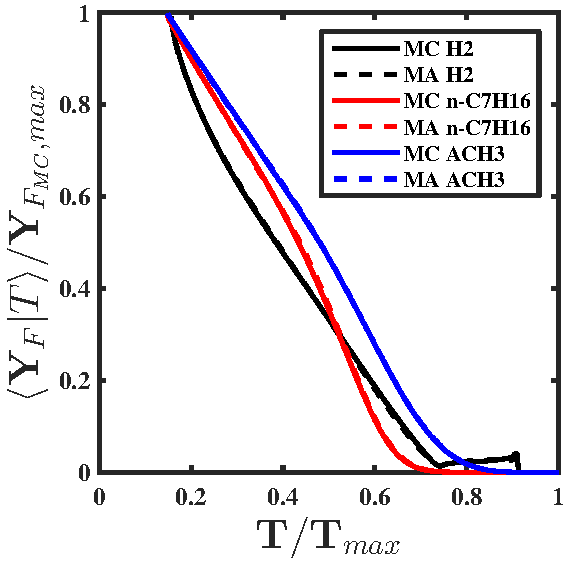
\includegraphics[width=\textwidth]{condmean_massfrac.pdf}
        \caption{}\label{A posteriori  (a)}
    \end{subfigure}
    \begin{subfigure}{0.33\textwidth}
        \centering
            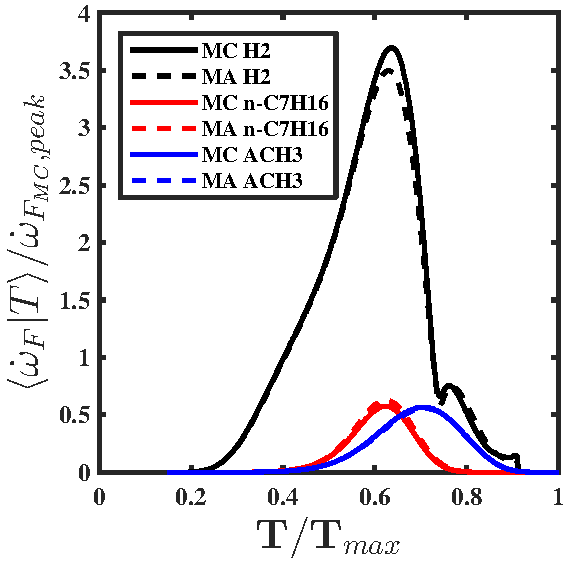
\includegraphics[width=\textwidth]{condmean_source.pdf}
        \caption{}\label{A posteriori (b)}
    \end{subfigure}
    \begin{subfigure}{0.33\textwidth}
        \centering
            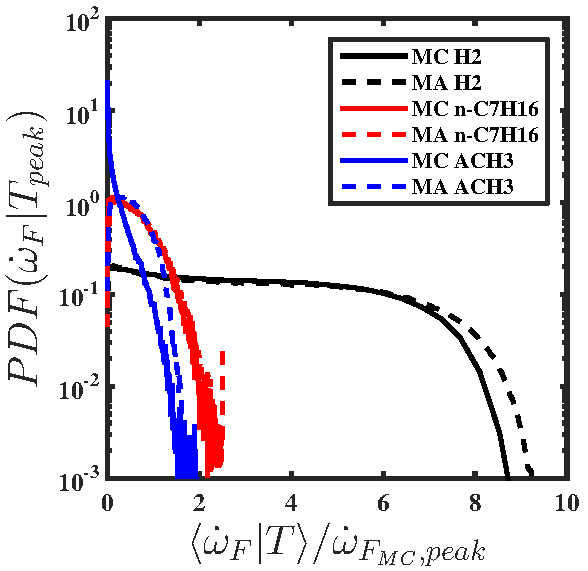
\includegraphics[width=\textwidth]{condmean_source_PDF.pdf}
        \caption{}\label{A posteriori (c)}
    \end{subfigure}
  \caption{\textcolor{blue}{Turbulence statistics for the three-dimensional premixed, turbulent flames, showing conditional means of (\subref{A posteriori  (a)}) fuel mass fraction (\subref{A posteriori (b)}) and source term as functions of flame temperature, as well as (\subref{A posteriori (c)}) the PDF of the source term at $T_{peak}$ \textcolor{red}{!!! Define $T_{peak}$!!!}.  All plots are normalized by their peak multicomponent values from one-dimensional flat flames.} \textcolor{red}{FIX PLOTS}}\label{A posteriori}
\end{figure*}

The observed differences in the calculated conditional means of the fuel mass fraction and consumption rate are small.
For all three simulations the average difference between the conditional means for the mixture-averaged and multicomponent cases are less \textcolor{red}{than \SI{3}{\%}.}
\textcolor{red}{!!! JS: To check data on 3D MA H2!!!} \textcolor{red}{The one exception to this consistency is in the hydrogen/air flames for a normalized temperature greater than 0.75, where the relative differences in the conditional means of the mass fraction are as much as \textcolor{red}{\SI{20}{\%}} between the mixture-averaged and multicomponent models.}
\textcolor{red}{!!! JS: Alter if conditional means still disagree!!!}  The agreement between the mixture-averaged and multicomponent results also extends into super-adiabatic regions of the hydrogen/air flame.
These super-adiabatic regions, also called ``hot spots'', are a result of differential diffusion effects, and have been predicted both in theoretical studies \cite{Williams:1985}, as well as in numerical analyses of lean hydrogen/air mixtures, e.g., \cite{Day:2009,AspdenJFM:2011,Aspden:2015}.

The a posteriori results using three-dimensional turbulent flames demonstrates that the small differences observed in the diffusion mass fluxes in Section \ref{sec:aprioriresults} do not significantly impact local quantities of the flame within the simulated broadened reaction zone regime.

\section{Conclusions}\label{sec:conclusions}
This article presents an a priori and a posteriori assessment of DNS mixture-averaged and multicomponent species diffusion models for two-dimensional unsteady hydrogen/air, and three-dimensional, turbulent, premixed, freely propagating flames considering hydrogen, n-heptane, and toluene fuel/air mixtures.
The mixture-averaged model was shown to accurately reproduce the relative direction and magnitude of the flux vectors in a priori analyses.  
The observed differences were quantified through statistical errors in regions where diffusion processes are important.  
While extending the analysis to the full domain does increase the discrepancy in both the relative angle and diffusion flux magnitude, these regions of increased relative error have less impact on the transport of species due to reduced diffusion fluxes.
This disagreement is expected and is due to the numerical relationship of the mixture-averaged and multicomponent diffusion fluxes to the species gradient but does not significantly impact simulation accuracy and fidelity.
A posteriori analyses also indicates that turbulent statistics, such as conditional means of the fuel mass fraction and consumption rates, are well predicted using the mixture-averaged diffusion model.
For the presented simulations, these conclusions suggest the mixture-averaged diffusion model is sufficient, and appropriate for DNS of three-dimensional, premixed turbulent flames in a moderate to high Karlovitz number regime.
% However, despite these results, there is insufficient data to draw firm conclusions on the accuracy and appropriateness of mixture-averaged assumptions for all flames.
% This result, although impactful is limited to a subset of turbulent flame within the high Karlovitz regime, additional data is needed to evaluate the appropriateness of the mixture-averaged assumption for different fuels, namely, oxi-fuels, multicomponent-hydrocarbon fuels, high pressure flames, and mechanisms with a greater number of species are needed to determine the.

\section*{Acknowledgments}
\label{Acknowledgments}
This material is based upon work supported by the National Science Foundation under Grant No.\ 1314109-DGE.
This research used resources of the National Energy Research Scientific Computing Center, a DOE Office of Science User Facility supported by the Office of Science of the U.S.\ Department of Energy under Contract No.\ DE-AC02-05CH11231.



%% References can be added with or without bibTeX database
%%
%% References with bibTeX database:
%% Note that the PROCI references style is considered Elsevier non-standard.
%% The original Elsevier bibliography style, elsarticle-num.bst prints paper titles as part of the references, which is different from 
\bibliography{bibliography.bib} %%User-specified
\bibliographystyle{elsarticle-num-PROCI.bst}

%% References without bibTeX database:
%%
% \begin{thebibliography}{99}
% \bibitem{Westbrook_1984} C. Westbrook, F. Dryer, Progress in Energy and Combustion Science 10 (1984) 1--57.
% \bibitem{Peters_2002} N. Peters, G. Paczko, R. Seiser, K. Seshadri, Combustion and Flame 128 (2002) 38--59.
% \end{thebibliography}

\end{document}

%%
%% End of file `template.tex'.
